\documentclass[a4paper,two side]{report}

%% Language and font encoding
\usepackage[english]{babel}
\usepackage[utf8x]{inputenc}
\usepackage[T1]{fontenc}


%% Sets page size and margins
\usepackage[a4paper,top=2cm,bottom=2cm,left=3cm,right=3cm,marginparwidth=2cm]{geometry}
%1.75cm
\usepackage{comment}
% makes the page borders visible
%\usepackage{showframe}

%% Useful packages
\usepackage{amsmath}
\usepackage{graphicx}
\usepackage[colorinlistoftodos]{todonotes}
\usepackage[colorlinks=true, allcolors=blue]{hyperref}

\usepackage[rightcaption]{sidecap}

\usepackage{wrapfig}

% this alters "before" spacing (the second length argument) to 0
\usepackage{titlesec}

\usepackage{lipsum}
\usepackage{listings}

\title{Project Title}

\begin{document}

\renewcommand{\baselinestretch}{1.5}

\begin{titlepage}

\newcommand{\HRule}{\rule{\linewidth}{0.5mm}} % Defines a new command for the horizontal lines, change thickness here

\center % Center everything on the page

\vspace*{\fill}\begin{center}
 
%----------------------------------------------------------------------------------------
%	HEADING SECTIONS
%----------------------------------------------------------------------------------------\
\textsc{\Huge \textbf {Goldsmiths}}\\ % Name of your university/college
\textsc{\small University of London}\\[1.5cm] % Name of your university/college
\textsc{\Large MSc Computer Games Programming}\\[0.5cm] % Major heading such as course name
\textsc{\large Department of Computing}\\[0.5cm] % Minor heading such as course title

%----------------------------------------------------------------------------------------
%	TITLE SECTION
%----------------------------------------------------------------------------------------
\makeatletter
\HRule \\[0.4cm]
{ \huge \bfseries \@title}\\[0.1cm] \large Procedural generation of cities using L System
\HRule \\[1.5cm]
 
%----------------------------------------------------------------------------------------
%	Student Details
%----------------------------------------------------------------------------------------
\Large \emph{Student Details:}\\ [0.2cm]
\large Sravan Kumar \textsc{Kairamkonda}\\[0.2cm]
\large 33673727\\[0.2cm]
\large skair001@gold.ac.uk\\[2cm] % Your name


%----------------------------------------------------------------------------------------
%	DATE SECTION
%----------------------------------------------------------------------------------------

{\large \today}\\[2cm] % Date, change the \today to a set date if you want to be precise

%\vfill % Fill the rest of the page with white space

\end{center}\vspace*{\fill}
\end{titlepage}

\renewcommand{\baselinestretch}{1}

%\section*{Brief}
1. You propose and realise a project in small teams (normally 2 or 3 students per team from the module). If you cannot (easily) form a group, contact me by email with your preferred topic.\newline \newline
2. You only need ONE submission PER GROUP.\newline \newline
3. Do put a READ ME.text saying : who (else)is on the team, title of project.\newline \newline
4. A link to your code repository will be just fine (e.g. on a GitHub space).\newline \newline
5. One video per group: a link to Vimeo/YouTube/etc. is fine; uploading your video (unless very large) should be possible too on the VLE.\newline \newline
6.Video can be short (e.g. 30 secs); one minute is likely plenty; longer ones should have a good narrative. (think: can I re-use this for my portfolio?)\newline \newline
7.Report (one per group): recommended you use a LaTeX format/tool (e.g. LyX, TeX maker, Overleaf, etc.), but you may use your favorite word processor of course. Should have the following parts/sections as a minimum:\newline \newline

\section*{Structure of the Report}
1. Title page (with at least names, course title/number, project title, date, logo or illustrative picture/teaser)\newline \newline
2. Introduction\newline \newline
3. Background : other works related to yours? summary/brief historical view on the subject (as  it relates to graphics or games or computing/maths).\newline \newline
4. Method: your work, description, decisions made, goals.\newline \newline
5. Team : how the project was managed, share of work, tasks, interactions\newline \newline
6. Results (put some visuals; link (URL) to your video)\newline \newline
7. Discussion or Conclusion (problems encountered, lessons learned, ideas, future work/improvements/features, ...)\newline \newline
8. Bibliography (at least 5 solid references).\newline \newline
9. Appendices : optional (more visuals, pseudo code, architecture, UI details, etc.)\newline \newline
10. NB : Teams details (members, selected topics) will appear later on.\newline 


\renewcommand{\baselinestretch}{1.5}

\begin{Large}

\begin{abstract}
\Large The development of video game is a complex system of auto generated data where it  created on run-time. There are few them that plays key role in the development process which are cities where the most of the gameplay interactions are used against the player. The creation of urban areas are deconstructed with different aspects mainly are roads and buildings around the area. We propose L-systems to generate roads, buildings and trees to randomize everything whenever they are loaded.\\[1cm]
\textbf{\textit{Key words}}: L Systems, Procedural Generation and Game Development
\end{abstract}

\tableofcontents
\thispagestyle{empty}

\end{Large}

% There are used remove space after and before paragraphs
\titleformat{\chapter}[display]
  {\normalfont\bfseries\Huge}
  {}
  {0pt}
  {}

\titlespacing{\chapter}
  {0pt}
  {-80pt}
  {0pt}
 
 % This is used to remove space before a paragraph
\setlength{\parindent}{0pt}

\cleardoublepage% ensures that the page numbering will change on a recto page
\pagenumbering{arabic}

\begin{Large}

\chapter{Project Details}

\vspace{1cm}

\begin{Large}

GitHub link \newline 
\url{https://github.com/YesItsSKM/Coursework-2}

\vspace{1cm}

Output video link \newline
\url{https://www.youtube.com/watch?v=-W7zt8181Zo&ab_channel=marian519 }

\end{Large}
\chapter{Introduction}

\Large The modern games production needs auto generated city which is a intensive task and everything represents the time period  of the game. The player spends most of the time in the environment with many interaction in the story along with gameplay mechanics\cite{abrahamcity}.The production quality is directly impacts on the cost of the project and final output team requires several artists and 3d model artists in order to develop the cities.

\vspace{0.5cm}

\Large Procedural generation is becoming more in the video games where as a lot of games are implementing the complex environments in the applications. Video games players wants to experience something new whenever they come to game. L System are extensively used to model plant ecosystems described in \cite{parish2001procedural}. The objective is simulate the roads, houses and trees using L-System algorithm. 


 
\chapter{Background}

\large 

\vspace{0.5cm}

\large
\chapter{Method}

\large We have used Unity Engine to generate the buildings, roads, and trees which is capable of handling the 3D procedural model with help of L System model. The basic models likes cities, roads and tress models are in their default orientation, whenever any object is instantiated in the scene, checks with the neighbour objects and sync to them. For instance: roads are different because there are intersections, dead ends and 3 way roads. Everything is calculated and verified with their neighbours models which generated through L System model\cite{abrahamcity}.

\vspace{0.5cm}

\large Buildings and trees are generated on bases of the road layout because they are needed to spawned beside the roads, similarly, trees are created with the equal subsequent distance among houses and also depends on the length of the street. The figure \ref{fig:flowchart} shows the flow of the model while generating it on run-time and described in the \cite{abrahamcity} an iterative process where graphics is interpreted with the strings. Some include of the stochastic rules a letter is replaced by the string with a probability of rules and angles.   

\begin{figure}[h]
\caption{Flow chart of a L System model}
\label{fig:flowchart}
\vspace{0.3cm}
\centering
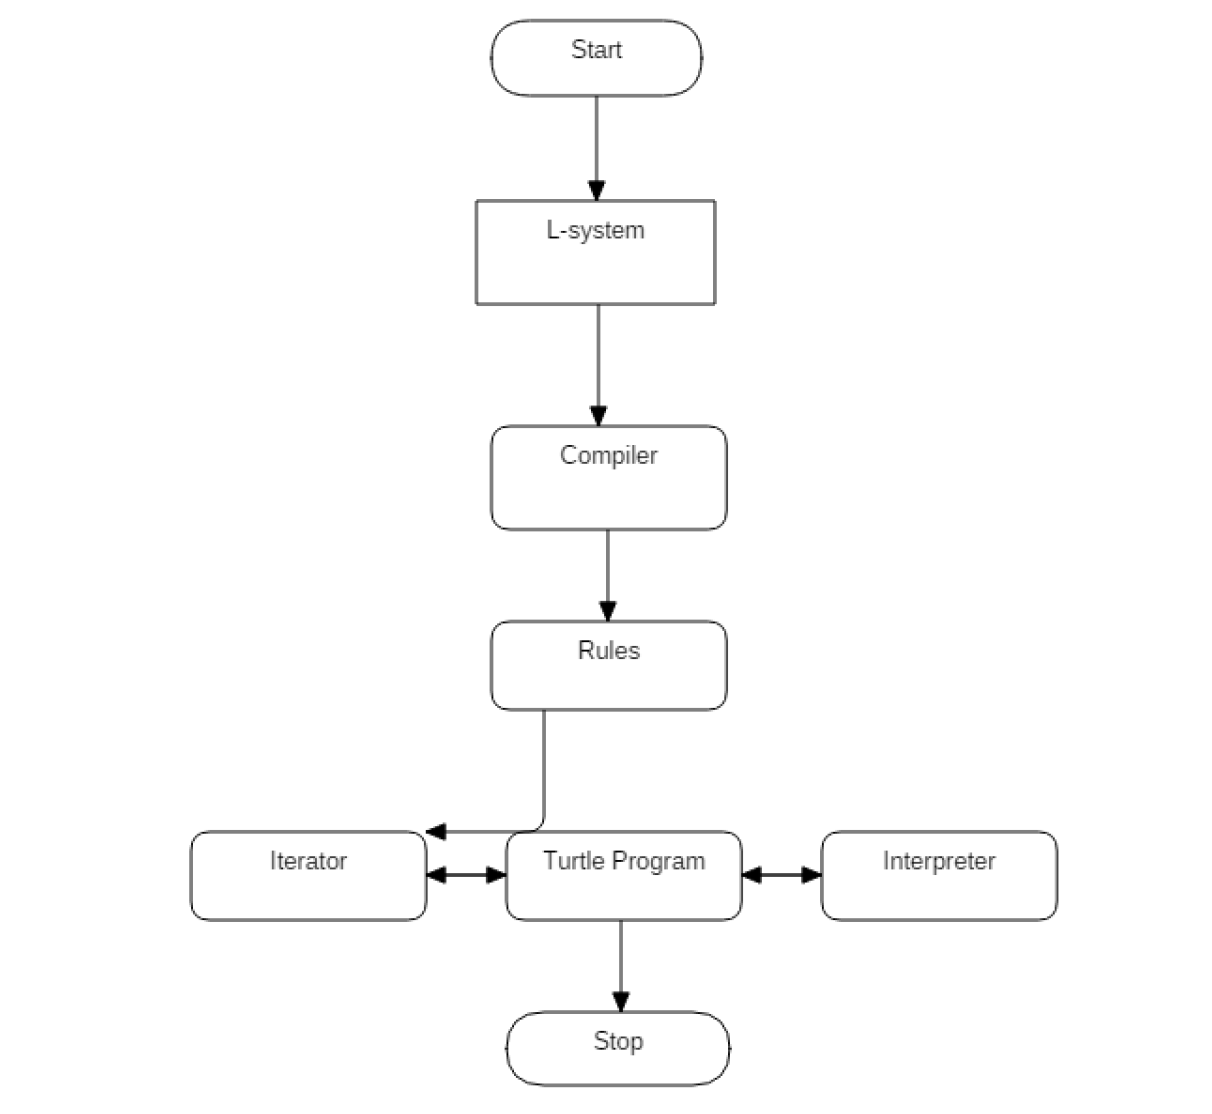
\includegraphics[width=0.6\textwidth]{3. method/Lsystem Flow Chart.png}
\end{figure}
\chapter{Team}

\large The objective of the projects are divided into three different tasks. The procedural generation of roads is assigned \textbf{Sravan Kairamkonda}, Placing houses are assigned to \textbf{Binto Bino} and  \textbf{Shubham Maurya} is assigned to placing Trees and adding animation.

\vspace{0.5cm}

\large The procedural generation of roads is generated with the L Systems where rules are used to create random roads. The roads are mapped with the based on the 3 way, 4 way and road ends \cite{galin2010procedural}.The algorithm divides the string into the characters where every character represents the road layout and its orientation the game world.
\chapter{Results}


\large Here we present some results of the output from the Unity Engine that are  auto generate output using L system which is shown on figure \ref{fig:road}, Road generated with in less than 2 second as the whole path is calculated with rules of string and some of them are ignored to create more randomization.

\begin{figure}[h]
\caption{Example of a random generated road using L system}
\label{fig:road}
\vspace{0.3cm}
\centering
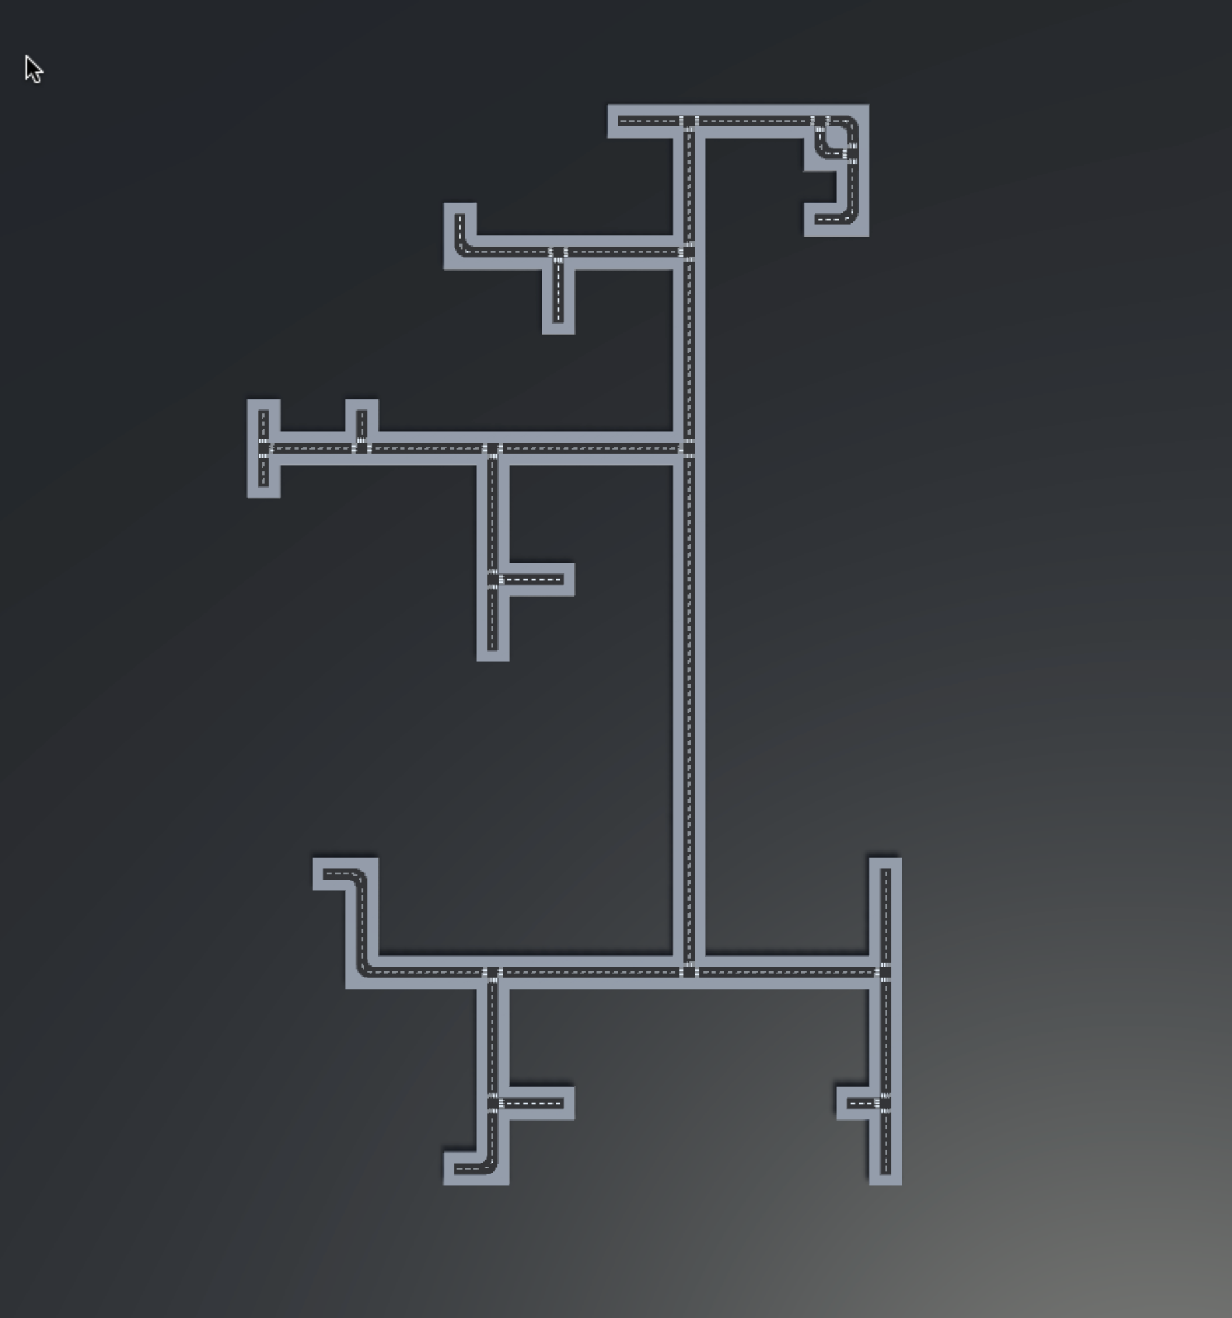
\includegraphics[width=0.6\textwidth]{5. results/Road Outpu.png}
\end{figure}

\renewcommand{\baselinestretch}{1.5}
\begin{scriptsize}
\begin{lstlisting} [language=C++, frame=single]
/// <summary>
/// Generates the string 
/// </summary>
/// <param name="newWord">Everything adds upto this word </param>
/// <param name="c">each character in the rule</param>
/// <param name="iterationIndex">number of iterations </param>
private void ProcessRulesRecursivelly(StringBuilder newWord, char c, int iterationIndex)
{
    foreach (var rule in rules)
    {
        if(rule.letter==c.ToString())
        {
            if (randomIgnoreRuleModifier)
            {
                if (Random.value < chanceToIgnoreRules && iterationIndex > 1)
                {
                    Debug.Log("Rule Ignored");
                    return;
                }
            }
            newWord.Append(GrowRecursive(rule.GetResult(), iterationIndex + 1));
        }
    }
}
\end{lstlisting}

\end{scriptsize}

\renewcommand{\baselinestretch}{1.5}

\large Shown in figure \ref{fig:road} the models of road are textured before are brought in to the unity so they are placed based on the direction that adds up to the either side of the roads.
\chapter{Conclusion}
\large The report presents the simplest form of generating cities which have a basic architecture like roads, buildings and trees which can be used to used generate them for the other objects in the game world. For instance, trees generating can be used to recreate the street lights and sign boards on the roads.

\vspace{0.5cm}

\large The system uses the GPU for the faster results that can be load the whole layout in a few seconds that helps to check the feel of the game as well as the art assets for the any prototype for the games and also for previsualization for the movies. The procedural generation saves a lot of time for the assets creation process.

\titleformat{\chapter}[display]
  {\normalfont\bfseries\Huge}
  {}
  {0pt}
  {}

\titlespacing{\chapter}
  {0pt}
  {0pt}
  {0pt}
  
\bibliographystyle{siam}
\bibliography{bibs/sample}

\appendix
\chapter{First Appendix}

\end{Large}

\end{document}